% ------------------------------------------------------------------------------
% TYPO3 CMS 7.4 - What's New (German Version)
%
% @author	Patrick Lobacher <patrick@lobacher.de> and Michael Schams <schams.net>
% @license	Creative Commons BY-NC-SA 3.0
% @link		http://typo3.org/download/release-notes/whats-new/
% @language	German
% ------------------------------------------------------------------------------
% LTXE-CHAPTER-UID:		0dbe76ce-5948c314-454b95fd-543cb62c
% LTXE-CHAPTER-NAME:	Backend User Interface
% ------------------------------------------------------------------------------
% LTXE-SLIDE-START
% LTXE-SLIDE-UID:		8080f469-3c5592f0-dc25ad87-894c2648
% LTXE-SLIDE-TITLE:		Feature: #48947 - Avatars for backend users
% LTXE-SLIDE-REFERENCE:	Feature-48947-AvatarsForBackendUsers.rst
% ------------------------------------------------------------------------------
\begin{frame}[fragile]
	\frametitle{Backend User Interface}
	\framesubtitle{Avatare für Backend Benutzer}

	Backend Benutzer können nun Avatare festlegen.
	Diese werden in den Benutzereinstellungen gepflegt und beispielsweise oben neben dem Anmeldenamen
	oder in den Benutzerlisten angezeigt.

	\begin{figure}
		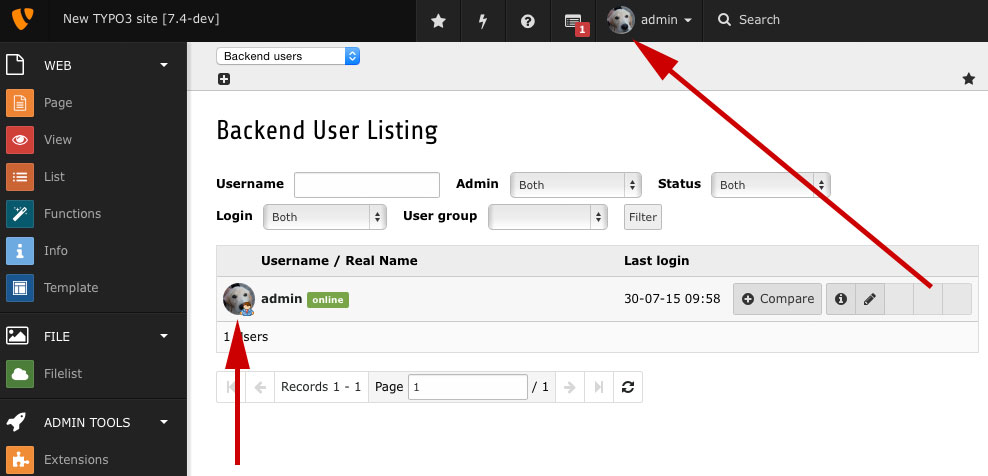
\includegraphics[width=0.9\linewidth]{BackendUserInterface/48947.jpg}
	\end{figure}

\end{frame}

% ------------------------------------------------------------------------------
% LTXE-SLIDE-START
% LTXE-SLIDE-UID:		b0f7e15a-7cc72aaa-79738ec7-643c5cec
% LTXE-SLIDE-TITLE:		Feature: #56133 - Replace file feature for fal file list
% LTXE-SLIDE-REFERENCE:	Feature-56133-ReplaceFileFeatureForFalFileList.rst
% ------------------------------------------------------------------------------
\begin{frame}[fragile]
	\frametitle{Backend User Interface}
	\framesubtitle{Dateien ersetzen}

	Es ist nun möglich, Dateien in der FAL Dateiliste zu \textbf{ersetzen}.
	Hierzu muss die "Erweiterte Ansicht" aktiviert sein.
	Je nach Bedarf kann der bisherige Dateinamen beibehalten oder der neue verwendet werden.

	\begin{figure}
		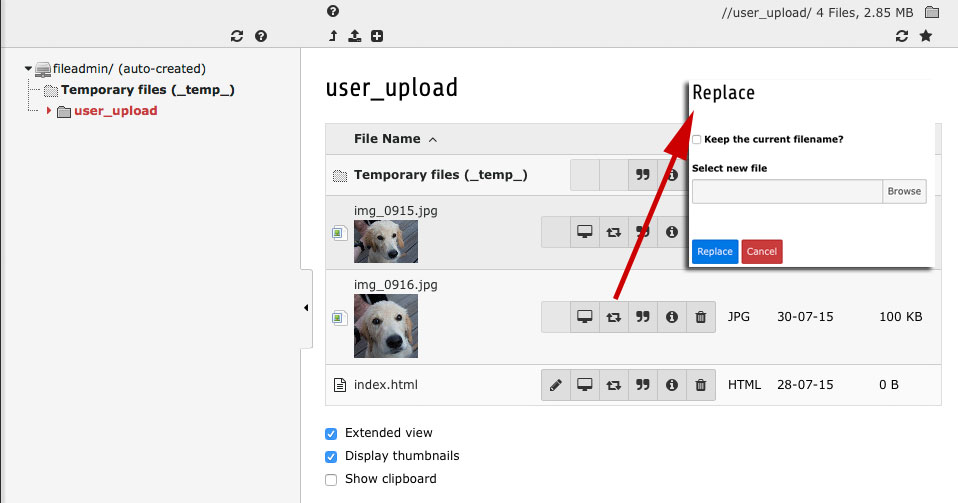
\includegraphics[width=0.75\linewidth]{BackendUserInterface/56133.jpg}
	\end{figure}

\end{frame}

% ------------------------------------------------------------------------------
% LTXE-SLIDE-START
% LTXE-SLIDE-UID:		613354cc-9475feef-bec620c5-31170549
% LTXE-SLIDE-TITLE:		Feature: #67574 - Display online status in backend user list
% LTXE-SLIDE-REFERENCE:	Feature-67574-DisplayOnlineStatusInBackendUserList.rst
% ------------------------------------------------------------------------------
\begin{frame}[fragile]
	\frametitle{Backend User Interface}
	\framesubtitle{Onlinestatus anzeigen}

	Im Modul "Backend Benutzer" wird nun angezeigt, ob ein Benutzer momentan online ist.

	\begin{figure}
		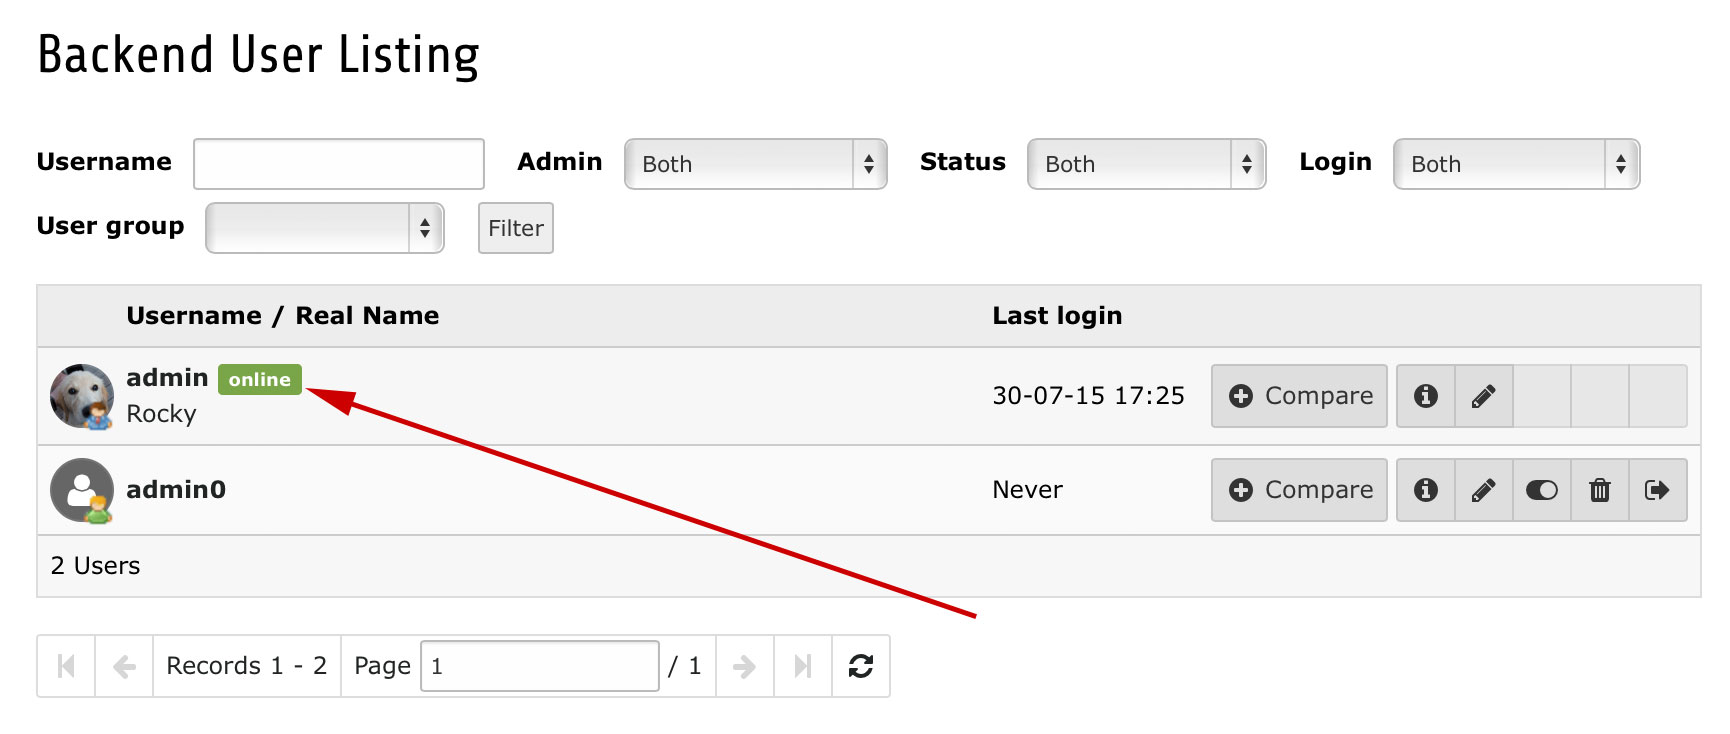
\includegraphics[width=0.9\linewidth]{BackendUserInterface/67574.jpg}
	\end{figure}

\end{frame}

% ------------------------------------------------------------------------------
% LTXE-SLIDE-START
% LTXE-SLIDE-UID:		00c93fe2-9d128591-20b71814-13556f43
% LTXE-SLIDE-TITLE:		FormEngine: Drop "Show secondary options"
% LTXE-SLIDE-REFERENCE:	https://forge.typo3.org/issues/67753
% ------------------------------------------------------------------------------
\begin{frame}[fragile]
	\frametitle{Backend User Interface}
	\framesubtitle{Zweite Optionspalette entfernt}

	Die Checkbox "Show secondary options (palettes)" sowie die TSconfig \texttt{options.enableShowPalettes}
	und die zugehörigen TCA-Einstellungen wurden entfernt. Die "Paletten" sind nun immer sichtbar und
	können nicht mehr ausgeblendet werden.

	\begin{figure}
		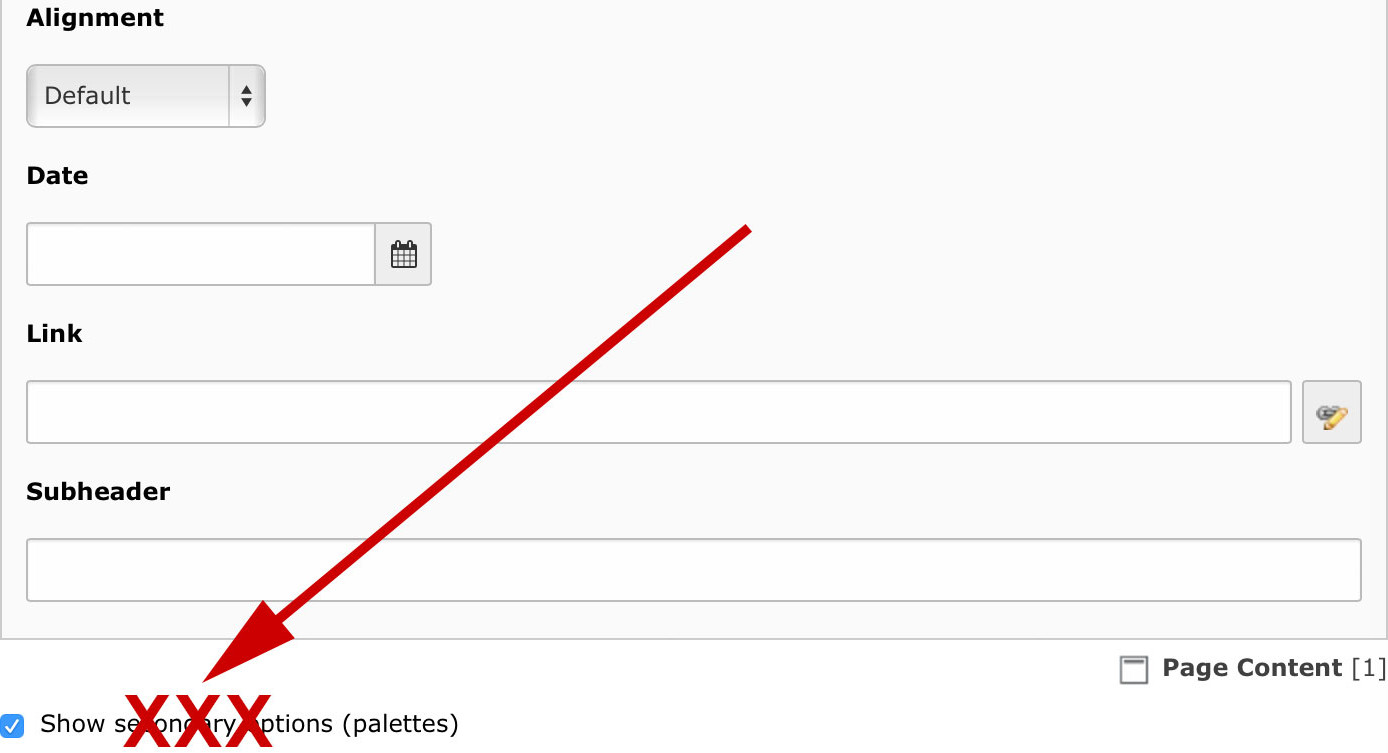
\includegraphics[width=0.6\linewidth]{BackendUserInterface/67753.jpg}
	\end{figure}

\end{frame}

% ------------------------------------------------------------------------------
% LTXE-SLIDE-START
% LTXE-SLIDE-UID:		bab4e93d-0a6d4612-41b2f67e-47c37ff7
% LTXE-SLIDE-TITLE:		Feature: #67578 - Add description-field for backend-users
% LTXE-SLIDE-REFERENCE:	Feature-67578-AddDescriptionFieldForBeUsers.rst
% ------------------------------------------------------------------------------
\begin{frame}[fragile]
	\frametitle{Backend User Interface}
	\framesubtitle{Beschreibung für Backend Benutzer}

	Backend Benutzer können nun auch eine Beschreibung erhalten.

	\begin{figure}
		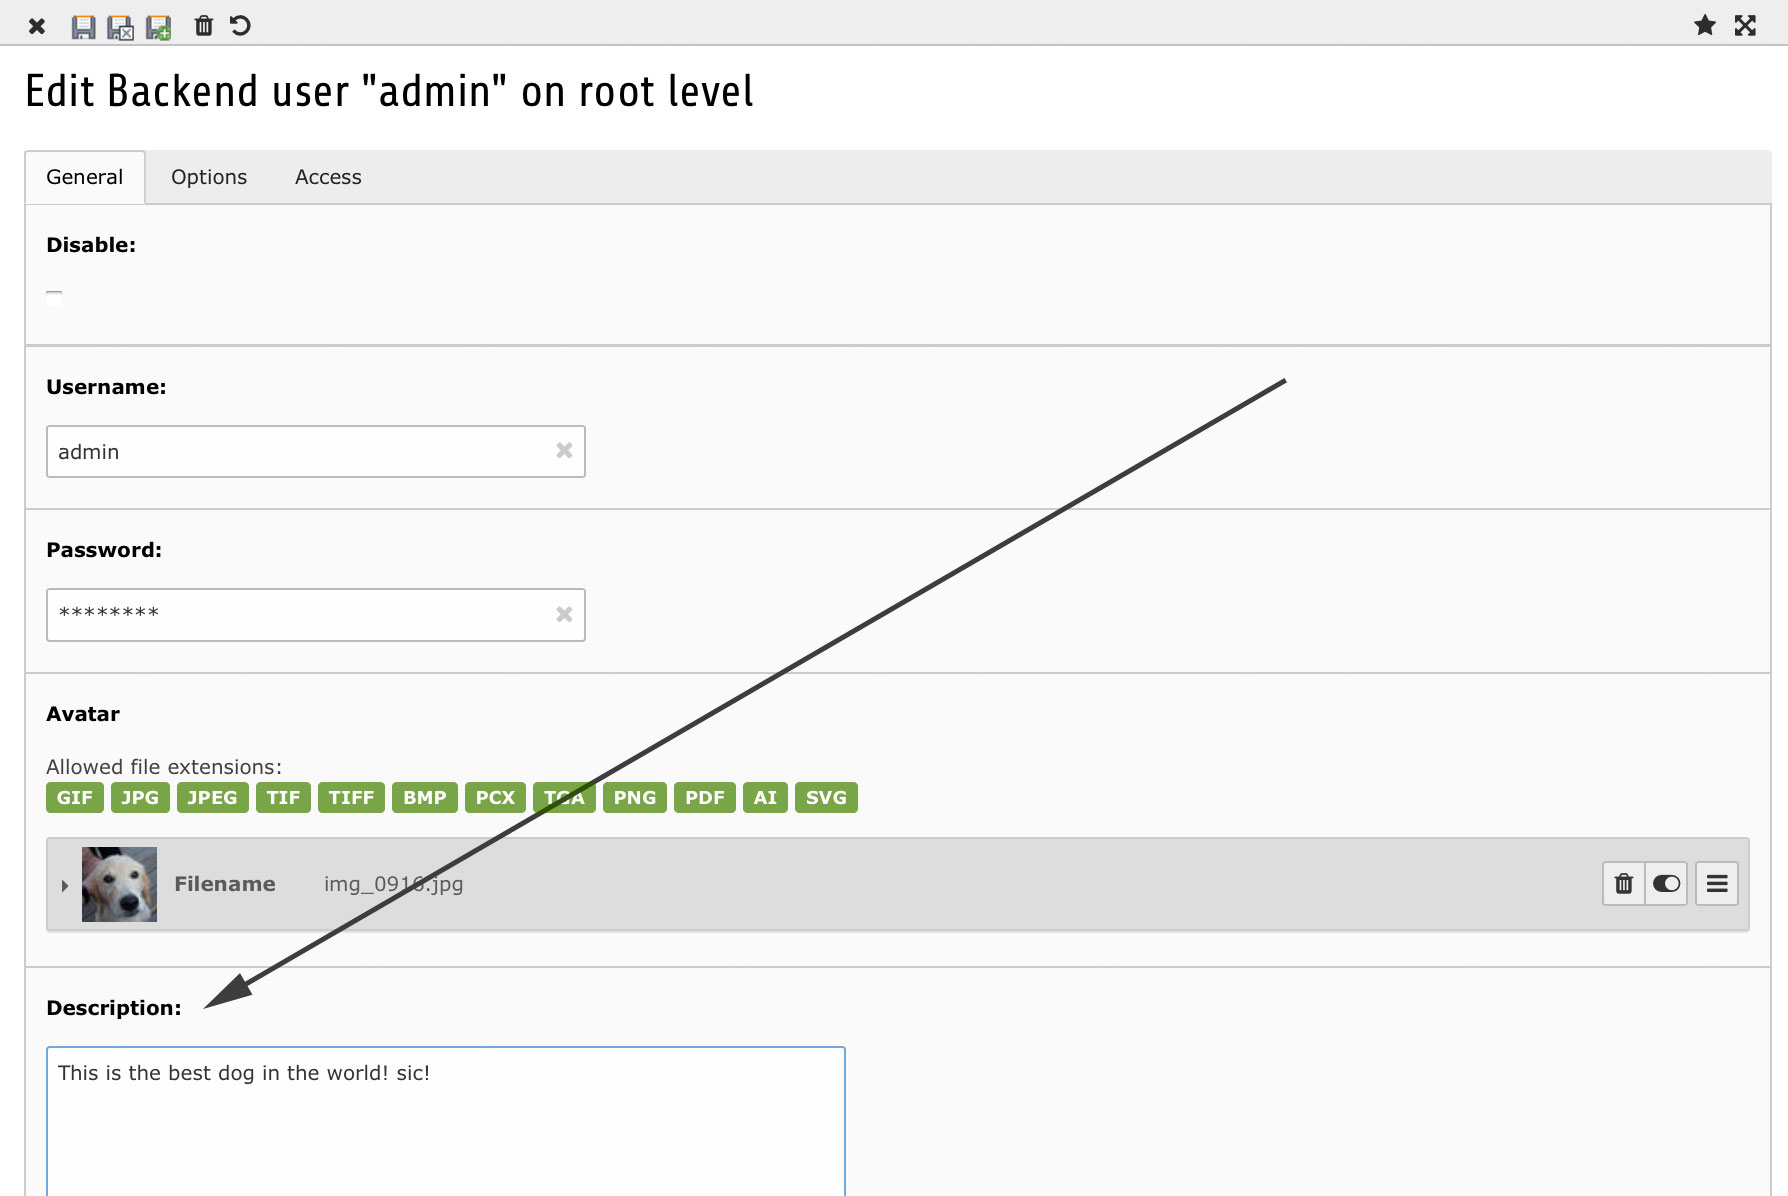
\includegraphics[width=0.7\linewidth]{BackendUserInterface/67578.jpg}
	\end{figure}

\end{frame}

% ------------------------------------------------------------------------------
% LTXE-SLIDE-START
% LTXE-SLIDE-UID:		649bd9ee-240381c8-950424ea-f032775b
% LTXE-SLIDE-TITLE:		Feature: #67603 - Introduce TCA > ctrl > descriptionColumn
% LTXE-SLIDE-REFERENCE:	Feature-67603-IntroduceTcaDescriptionColumn.rst
% ------------------------------------------------------------------------------
\begin{frame}[fragile]
	\frametitle{Backend User Interface}
	\framesubtitle{Beschreibung im Backend anzeigen}

	Über die TCA-Einstellung \texttt{['TCA']['ctrl']['descriptionColumn']} kann eine Spalte ausgewählt werden
	(meist \texttt{description}), die eine Beschreibung enthält.
	Ist diese vorhanden, wird der Inhalt beispielsweise im Listenmodul angezeigt.

	\begin{figure}
		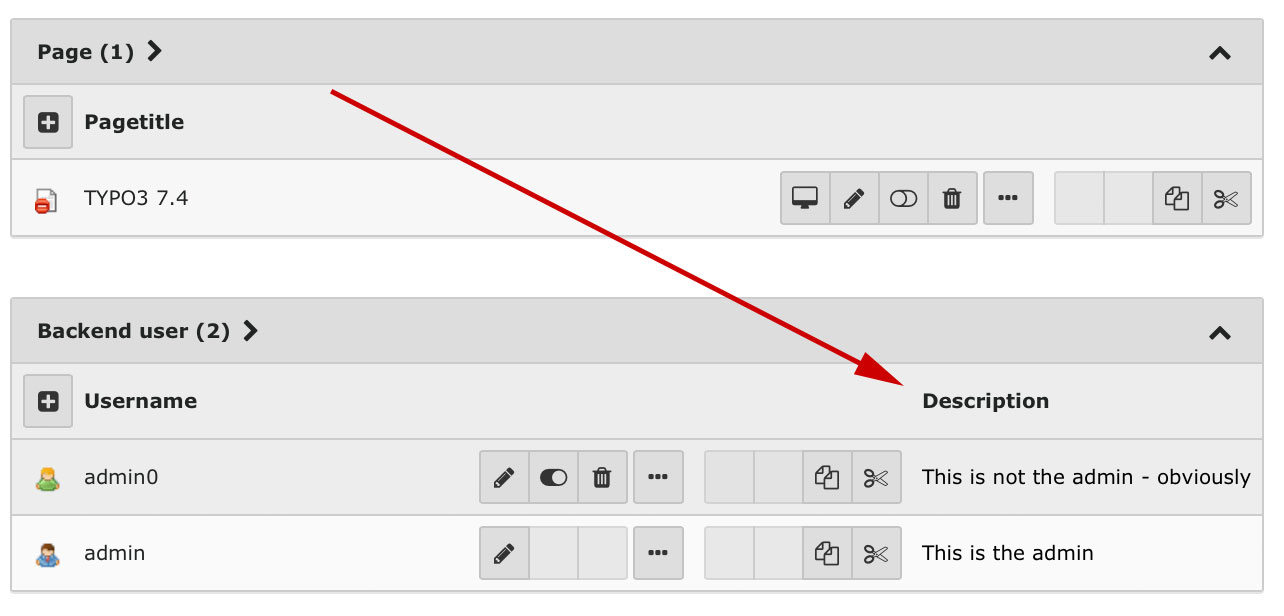
\includegraphics[width=0.7\linewidth]{BackendUserInterface/67603.jpg}
	\end{figure}

\end{frame}

% ------------------------------------------------------------------------------
% LTXE-SLIDE-START
% LTXE-SLIDE-UID:		2eeaec46-1929743b-8e6f9285-13d20d3c
% LTXE-SLIDE-TITLE:		Feature: #59570 - Add description-field for filemounts
% LTXE-SLIDE-REFERENCE:	Feature-59570-AddDescriptionFieldForFilemounts.rst
% ------------------------------------------------------------------------------
\begin{frame}[fragile]
	\frametitle{Backend User Interface}
	\framesubtitle{Beschreibung für Filemounts}

	Filemounts können ebenfalls eine Beschreibung erhalten.

	\begin{figure}
		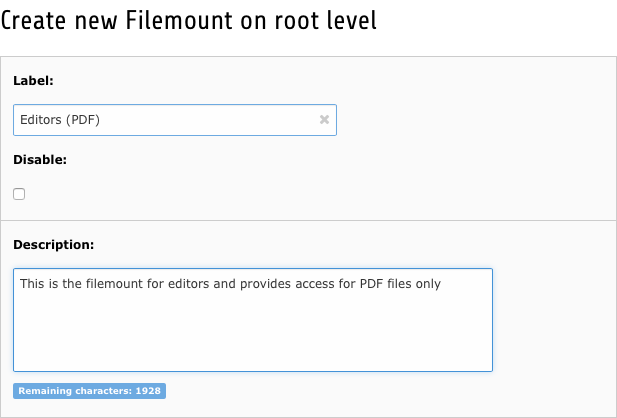
\includegraphics[width=0.66\linewidth]{BackendUserInterface/59570.png}
	\end{figure}

\end{frame}

% ------------------------------------------------------------------------------
% LTXE-SLIDE-START
% LTXE-SLIDE-UID:		879b1dda-9167d830-373f7457-0391ebee
% LTXE-SLIDE-TITLE:		Feature: #68197 - Show a dialog for existing files on upload
% LTXE-SLIDE-REFERENCE:	Feature-68197-ShowADialogForExistingFilesOnUpload.rst
% ------------------------------------------------------------------------------
\begin{frame}[fragile]
	\frametitle{Backend User Interface}
	\framesubtitle{Überschreiben Dialog beim Upload}

	Sofern bei einem Upload Dateien bereits auf dem Server existieren,
	werden in einem Dialog mehrere Optionen zur Auswahl angeboten.

	\begin{figure}
		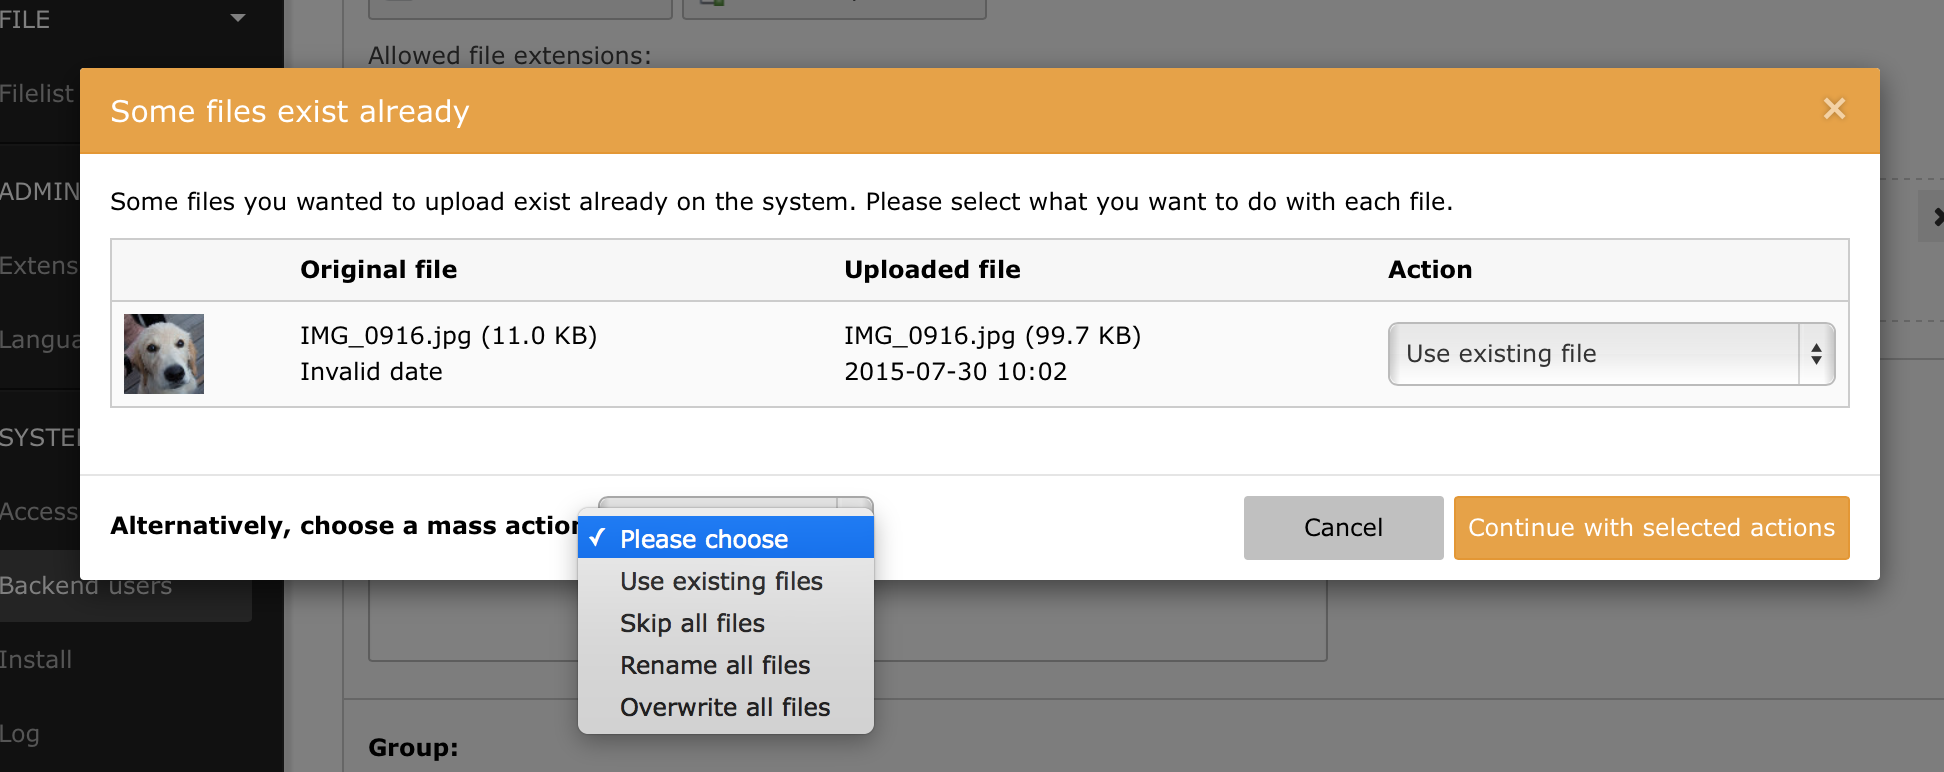
\includegraphics[width=0.9\linewidth]{BackendUserInterface/68197.png}
	\end{figure}

\end{frame}


% ------------------------------------------------------------------------------
% LTXE-SLIDE-START
% LTXE-SLIDE-UID:		f4baa7b8-2237ad1d-5c4be365-a845f207
% LTXE-SLIDE-TITLE:		Feature: #68218 - Lock edit for tt_content
% LTXE-SLIDE-REFERENCE:	Feature-68218-LockEditForTt_content.rst
% ------------------------------------------------------------------------------
\begin{frame}[fragile]
	\frametitle{Backend User Interface}
	\framesubtitle{Editieren von Inhaltselementen für Nicht-Admins einschränken}

	Inhaltselemente können jetzt für die Bearbeitung durch Nicht-Admins eingeschränkt werden
	(ähnliche Funktion die es bereits bei Seiten gibt).

	\begin{figure}
		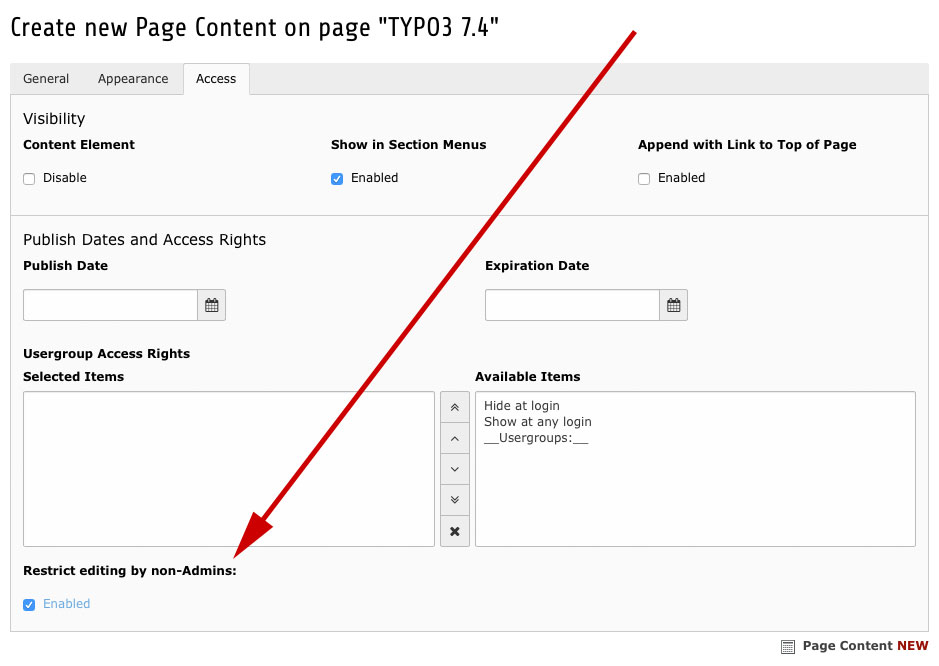
\includegraphics[width=0.6\linewidth]{BackendUserInterface/68218.jpg}
	\end{figure}

\end{frame}

% ------------------------------------------------------------------------------
% LTXE-SLIDE-START
% LTXE-SLIDE-UID:		bc83e40f-9b7bac03-ea5f07c4-be27eb56
% LTXE-SLIDE-TITLE:		Feature: #68315 - Include pageTSconfig file (1)
% LTXE-SLIDE-REFERENCE:	Feature-68315-IncludeAPageTSconfigFileInPagePropertiesLikeTSStaticTemplates.rst
% ------------------------------------------------------------------------------
\begin{frame}[fragile]
	\frametitle{Backend User Interface}
	\framesubtitle{Statische TSconfig Dateien (1)}

	In den Seiteneigenschaften können nun statische TSconfig Dateien eingebunden werden.

	\begin{figure}
		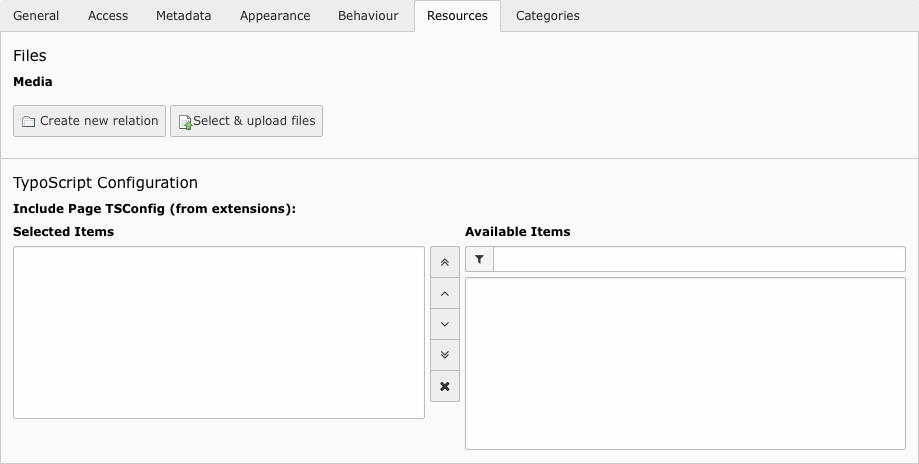
\includegraphics[width=0.8\linewidth]{BackendUserInterface/68315.png}
	\end{figure}

\end{frame}

% ------------------------------------------------------------------------------
% LTXE-SLIDE-START
% LTXE-SLIDE-UID:		9b7bac03-ea5f07c4-be27eb56-ac03e27e
% LTXE-SLIDE-TITLE:		Feature: #68315 - Include pageTSconfig file (2)
% LTXE-SLIDE-REFERENCE:	Feature-68315-IncludeAPageTSconfigFileInPagePropertiesLikeTSStaticTemplates.rst
% ------------------------------------------------------------------------------
\begin{frame}[fragile]
	\frametitle{Backend User Interface}
	\framesubtitle{Statische TSconfig Dateien (2)}

	% decrease font size for code listing
	\lstset{basicstyle=\tiny\ttfamily}

	Die TSconfig Dateien werden wie folgt registriert:

	\begin{lstlisting}
		\TYPO3\CMS\Core\Utility\ExtensionManagementUtility::registerPageTSConfigFile(
		  'extension_name',
		  'Configuration/PageTS/myPageTSconfigFile.txt',
		  'My special configuration'
		);
	\end{lstlisting}

\end{frame}

% ------------------------------------------------------------------------------
% LTXE-SLIDE-START
% LTXE-SLIDE-UID:		f8d888b1-b93dcf4a-e20b976e-9a5c277e
% LTXE-SLIDE-TITLE:		Feature: #68395 - Allow real copies of content elements into foreign languages
% LTXE-SLIDE-REFERENCE:	Feature-68395-AllowRealCopiesOfContentElementsIntoForeignLanguages.rst
% ------------------------------------------------------------------------------
\begin{frame}[fragile]
	\frametitle{Backend User Interface}
	\framesubtitle{Echte Sprachkopien}

	Es ist nun möglich, "richtige" Kopien von Inhaltselementen in Sprachversionen anzulegen
	(und nicht nur Referenzen).

	\begin{figure}
		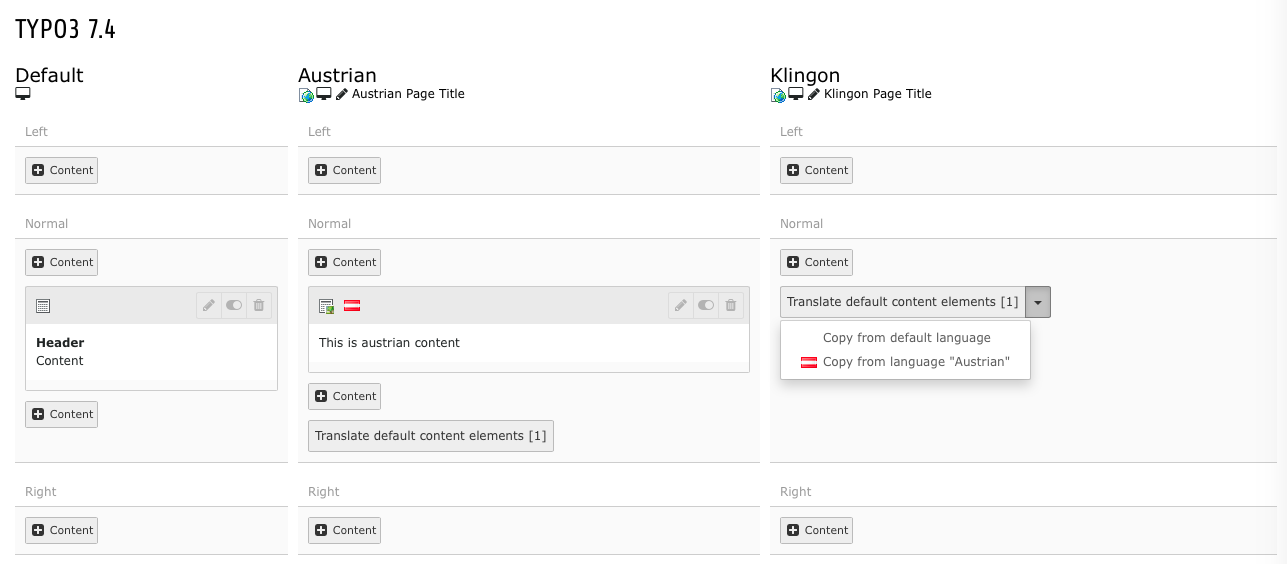
\includegraphics[width=0.9\linewidth]{BackendUserInterface/68395.png}
	\end{figure}

\end{frame}


